% \documentclass[sigconf,anonymous,review,timestamp]{acmart}
\documentclass[sigconf]{acmart}

%% Rights management information.  This information is sent to you
%% when you complete the rights form.  These commands have SAMPLE
%% values in them; it is your responsibility as an author to replace
%% the commands and values with those provided to you when you
%% complete the rights form.
\setcopyright{acmcopyright}
\copyrightyear{2023}
\acmYear{2023}
\acmDOI{XXXXXXX.XXXXXXX}

%% These commands are for a PROCEEDINGS abstract or paper.
\acmConference[Conference acronym 'XX]{Conference title}{January 01--02,
  1900}{Someplace, NY}
\acmPrice{15.00}
\acmISBN{978-1-4503-XXXX-X/18/06}

%%
%% Submission ID.
%% Use this when submitting an article to a sponsored event. You'll
%% receive a unique submission ID from the organizers of the event,
%% and this ID should be used as the parameter to this command.
\acmSubmissionID{123-A56-BU3}

%%
%% The majority of ACM publications use numbered citations and
%% references.  The command \citestyle{authoryear} switches to the
%% "author year" style.
%%
%% If you are preparing content for an event
%% sponsored by ACM SIGGRAPH, you must use the "author year" style of
%% citations and references.
%% Uncommenting
%% the next command will enable that style.
\citestyle{acmauthoryear}

%% To fix a margin violation bug, apparently due to poor hyphenation.
\hyphenation{Go-men-so-ro}
%% For introducing terms which have a special meaning in this work.
\newcommand{\jargon}[1]{\textit{#1}}

\begin{document}

\title{Coevolution of Camouflage}

%% Author
\author{Craig Reynolds}
\email{cwr@red3d.com}
\orcid{0000-0001-8203-712X}
\affiliation{%
  \institution{unaffiliated researcher}
  \country{USA}
}

\renewcommand{\shortauthors}{Craig Reynolds}

\begin{abstract}
  Camouflage in nature seems to arise from competition between predators who must find prey to survive, and prey who must avoid detection to survive. This work simulates a simplified, abstract model of this adversarial relationship. It looks at \textit{crypsis} through evolving prey camouflage patterns (as color textures) in competition with evolving predator vision which learns to locate camouflaged prey. The environment for this 2D simulation is provided by a set of photographs, typically of natural scenes. This simulation is based on an evolving population of predators and another of prey. The mutual conflict between these populations tends to produce both effective camouflage and skilled predators. This simulation provides a method for creating camouflage patterns for arbitrary backgrounds, and more significantly an experimental \textit{artificial life} model for investigating aspects of camouflage evolution in nature. All code and research notes are available on GitHub.
\end{abstract}

%%
%% Generate your CCSCML using http://dl.acm.org/ccs.cfm.
%%
\begin{CCSXML}
<ccs2012>
   <concept>
       <concept_id>10010147.10010341.10010349.10011810</concept_id>
       <concept_desc>Computing methodologies~Artificial life</concept_desc>
       <concept_significance>500</concept_significance>
       </concept>
   <concept>
       <concept_id>10010147.10010371.10010382.10010384</concept_id>
       <concept_desc>Computing methodologies~Texturing</concept_desc>
       <concept_significance>300</concept_significance>
       </concept>
   <concept>
       <concept_id>10010147.10010178.10010224</concept_id>
       <concept_desc>Computing methodologies~Computer vision</concept_desc>
       <concept_significance>300</concept_significance>
       </concept>
    <concept>
       <concept_id>10010147.10010178.10010224.10010245.10010246</concept_id>
       <concept_desc>Computing methodologies~Interest point and salient region detections</concept_desc>
       <concept_significance>300</concept_significance>
       </concept>
    <concept>
        <concept_id>10010147.10010257.10010293.10011809.10011813</concept_id>
        <concept_desc>Computing methodologies~Genetic programming</concept_desc>
        <concept_significance>300</concept_significance>
    </concept>
 </ccs2012>
\end{CCSXML}

\ccsdesc[500]{Computing methodologies~Artificial life}
\ccsdesc[300]{Computing methodologies~Texturing}
\ccsdesc[300]{Computing methodologies~Computer vision}
\ccsdesc[300]{Computing methodologies~Interest point and salient region detections} 
\ccsdesc[300]{Computing methodologies~Genetic programming}


%% Keywords
\keywords{camouflage, coevolution, nature, biology, predator, prey, vision, texture synthesis}

%% Teaser figure that appears on the top of the article.
\begin{teaserfigure}
    %% TODO note: use images without the “predator prediction crosshairs”.
    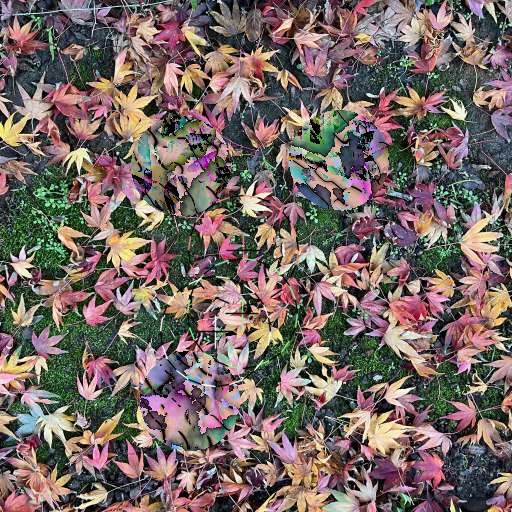
\includegraphics[scale=0.24]{images/20220918_step_7372.png}
    \hfill
    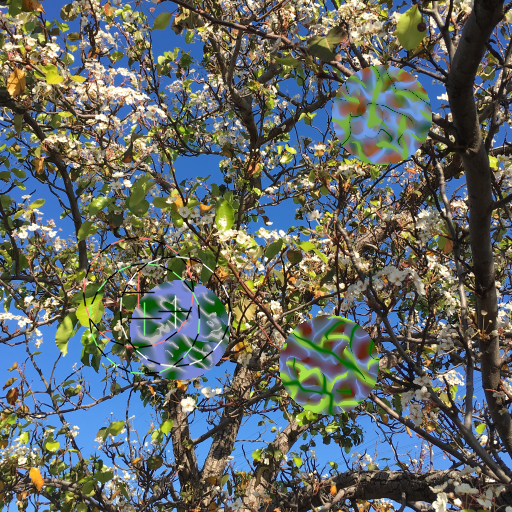
\includegraphics[scale=0.24]{images/20220926_step_6143.png}
    \hfill
    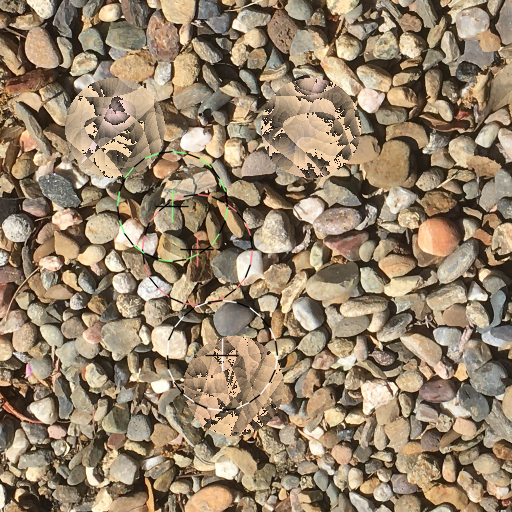
\includegraphics[scale=0.24]{images/20221003_step_3667.png}
    \hfill
    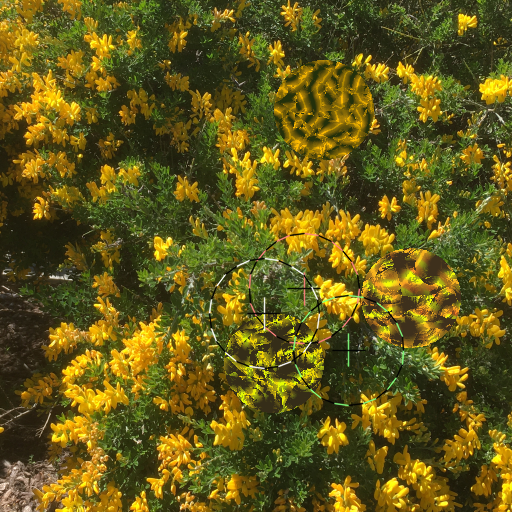
\includegraphics[scale=0.24]{images/20220930_step_6093.png}
    \caption{Photographs of natural textures, each overlaid with three camouflaged \textit{prey}. The prey are randomly placed 2D disks, each with its own evolved camouflage texture. (Note: for best results zoom into the digital version. [QQQ replace stand-in images]}
    \Description{Examples of camouflage textures produced by the simulation.}
    \label{fig:teaser}
    % \vspace{5mm} %5mm vertical space
    \vspace{3mm} % 3mm vertical space
\end{teaserfigure}

%% Lay out the single column “top matter” defined above.
\maketitle

\begin{figure*}
    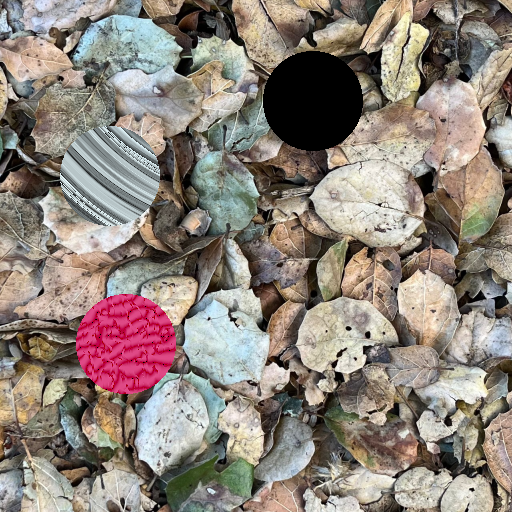
\includegraphics[scale=0.16]{images/20221016_step_969.png}
    \hfill
    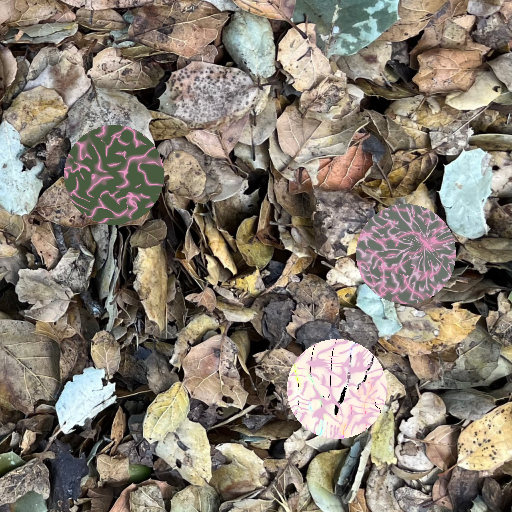
\includegraphics[scale=0.16]{images/20221016_step_1710.png}
    \hfill
    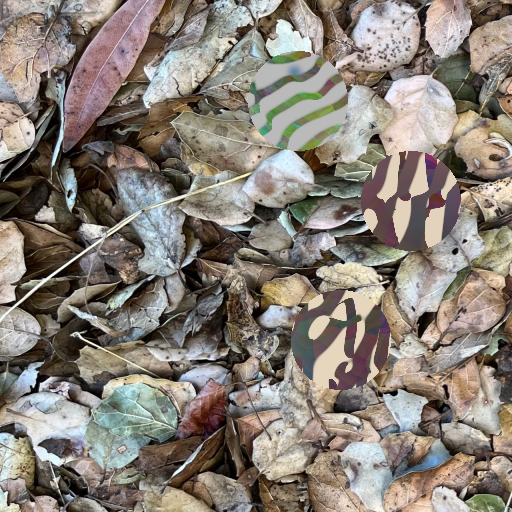
\includegraphics[scale=0.16]{images/20221016_step_2368.png}
    \hfill
    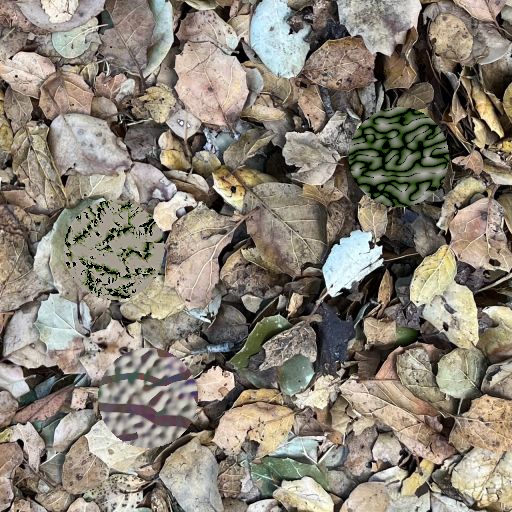
\includegraphics[scale=0.16]{images/20221016_step_3420.png}
    \hfill
    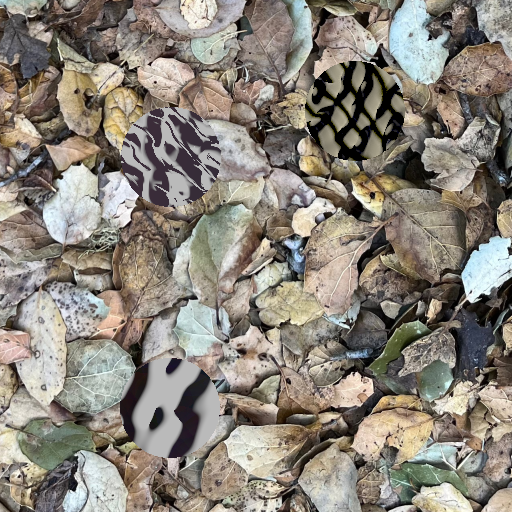
\includegraphics[scale=0.16]{images/20221016_step_4864.png}
    \hfill
    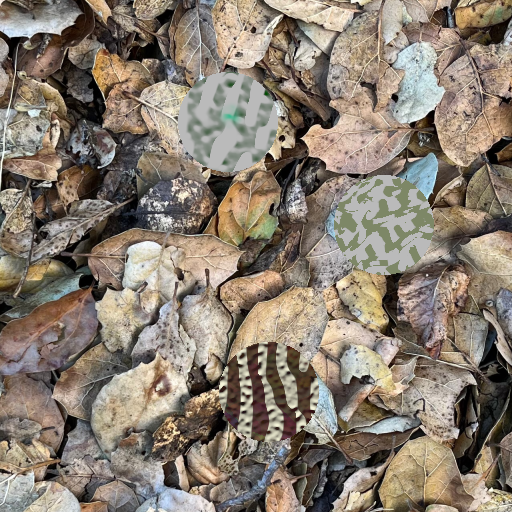
\includegraphics[scale=0.16]{images/20221016_step_5564.png}
    \caption{Evolution of the prey population over simulation time}
    \Description{Sequence of images showing evolution of prey population over simulation time.}
    \label{fig:time_sequence}
\end{figure*}

\section{Introduction}
This work aims to create a simplified and abstract 2d simulation model of the evolution of camouflage textures in nature. These camouflage patterns emerge in the interaction — the coevolution — of a population of \textit{prey} each with a candidate texture and a population of \textit{predators} each with a learned visual detector. The input to the simulation is a set of photos of a background environment. The prey evolve to be \textit{cryptic} (hard to see) against the background images. The predators evolve and learn to hunt the prey by locating their position within the 2D environment.
\par
Computational models of complex biological systems have several benefits. Constructing them, getting them to work as seen in nature, helps crystallize our thinking about natural phenomenon. Computational models also allow experimentation \textit{in silico} to help characterize complex natural systems.
\par
Following the approach of \citet{Reynolds2011} a population of prey, each with a synthetic camouflage texture, are evolved in response to negative selection by a predator seeking the prey most conspicuous against a given background. In that game-like interactive simulation, the predator was a human “player.” The simulation would display a photographic background image overlaid with camouflaged prey. The human predator would select, with a mouse click, the most conspicuous five of ten displayed prey. These “eaten” prey were removed from the population, and replaced by offspring created by genetic \textit{crossover} between surviving prey followed by \textit{mutation}. This simulation step was repeated around 2000 times.
\par
In the simulation described here, evolution of prey camouflage closely follows that earlier work. But here, the human-in-the-loop is replaced with a second population of predators, each based on a deep neural network. These CNN networks take an image as input and produce a prediction, an estimate, of where in the image the most conspicuous prey is location. The input to these neural nets is a a small RGB image (a 128x128x3 tensor: 49,152 floating point numbers) and the output is two floats, interpreted as an XY position relative to the image. 
\par
(Note that the images in this paper are rendered at 512² pixels and the prey disks have a diameter of 100 pixels. These images are downsampled to 128² for use by predator's vision CNNs.)
\par
A bit of explanation for the term “abstract model.” In artificial life models it is common to focus in detail on one aspect of a natural system. In the current model, it is the coevolutionary dynamics between prey camouflage and predator vision. To make this feasible, other levels of organization, are ignored, or assumed, or represented by a simple computation stand-in. So for example, the entire living organism that embodies these predators and prey, are simply assumed to exist, behaving as animals do, and are otherwise ignored. This model has a simple abstract representation of biological morphogenesis as programs in TexSyn's language for procedural texture synthesis. \textit{Genetic Programming} provides a simple model of evolution which acts on this “genetic” representation, creating new “offspring” textures through crossover and mutation. On the predator side, we ignore all of the animal's existence except for the key aspect of hunting behavior: looking at a scene and forming an opinion about where in the scene a prey is likely to exist. These predators can adapt to the appearance of an environment and the prey found there, by learning from its experience. Predators compete with each other on the basis of their ability to hunt prey and so eat. The details of evolution, morphogenesis, vision, and genetic representation are all completely unlike the natural world. The assumption is that they are sufficiently similar in effect to allow a plausible simulation of the natural system, producing analogous results, which may provide insights about the natural system.

\section{Related work}
This work can be seen as an extension of \citet{Reynolds2011} where the human predator there is replaced with an evolving population of procedural predators, whose hunting is based on a learning vision model. An earlier attempt at this approach, using coevolution and procedural predators was described by \citet{harrington_coevolution_2014}.
\par
Closely related work on learning surface textures to camouflage 3D objects within real 3D scenes is described for cubes using one technique in \citet{owens_camouflaging_2014} and for arbitrarily shaped 3D objects using an improved technique in \citet{guo_ganmouflage_2022}. In both cases, the 3D scene is described by a set of photos of it from various viewpoints. The textures mapped onto the object to be camouflaged must trade off being inconspicuous from all viewpoints in the scene.
\par
Other computer graphics work related to camouflage include detailed reproduction of coloration patterns on real animals \cite{de_gomensoro_malheiros_leopard_2020} and generation of visual puzzles incorporating camouflaged images \cite{chu_camo_image_2010} \cite{Zhang_Yin_Nie_Zheng_2020}. CamoEvo \cite{hancock_camoevo_2022} is a toolbox for authoring online camouflage evolution games (similar to \citet{Reynolds2011}) to study natural biological species.
\par
The procedural texture synthesis used here to generate camouflage patterns has a long history. This work is perhaps most directly inspired by \citet{perlin_image_1985} where images are rendered from purely procedural representation. [... maybe this should be in the section on texture synthesis? ... These textures are object-oriented so specific types are implemented as (c++) classes, with specific parameters stored in instances. The base class provides interfaces for operations such as returning a color for a given position on the (infinite) texture plane. ...] The combination of texture synthesis under control of a genetic algorithm goes back to \citet{sims_artificial_1991}, which in turn was inspired by the interactive biomorph evolution demo in \citet{dawkins_blind_1986}. [... Latham and Todd ...]
\par
Evolution is represented in this model using \jargon{genetic programming} (GP), a type of population-based evolutionary optimization algorithm, first described by \citet{cramer_representation_1985} and popularized by \citet{koza_genetic_1992}. GP is a variation of \jargon{genetic algorithms} (GA). GA traditionally uses a fixed length bit string as its genetic representation, while GP uses an arbitrarily-sized tree-shaped representation. GP trees conveniently map onto nested expressions in a domain specific language. Texture synthesis in this work is based on nested expressions of texture operators from the TexSyn library, see Figure \ref{fig:TexSyn_overview}. A prey population of these textures is optimized for camouflage effectiveness by GP using the selection pressure of a population of predators which serve to determine fitness. TexSyn is used with the \jargon{strongly typed} variant of Genetic Programming known as STGP \cite{montana_strongly_1995}, one of several grammar-based GP variants \cite{Mckay_2010}.
\par
The biological literature on camouflage and related topics is vast. A few starting points include: [... historical survey of campoouflage in nature ... \citet{thayer_concealing-coloration_1909}, early work on mathematical models of biological patterns \citet{turing_chemical_1952}, revisiting Turing's work with modern computation ... \citet{murray_how_1988},  ...how life evolves and learns... \citet{valiant_probably_2013}, QQQ find other basic bio references from my 2010 paper? ...]
\par
\subsection{Camouflaged object detection}
In the last several years, there has been burst of related research on \jargon{camouflaged object detection} (COD) in computer vision. See for example this well-curated list of COD publications by \citet{visionxiang_cod}. COD is part of predator behavior: detecting the presence of a camouflaged object. But these COD systems focus on \jargon{segmenting} the camouflaged object: finding a per-pixel mask of its projection in an image. A recent example, which surveys this topic and presents its own strong solution, is \citet{Zhang2022}. Others works on COD include some based on boundaries \cite{chen_boundary-guided_2022} \cite{sun_boundary-guided_2022}, an attempt to rank camouflaged objects by “conspicuousness” \cite{lv_cod_2022}, and a mixed-scale approach \cite{pang_zoom_2022}.
\par
COD attempts \textit{a priori} camouflage “breaking” — detecting the presence of well camouflaged objects — without learning either the background or the typical appearance of prey camouflage found in a given environment. That is, they seek to be a \jargon{generalist} predator, effectively using a strong form of \jargon{salience}. As summarized in \citet{Zhang2022}, COD is based on several labeled datasets (CHAMELEON, CAMO, and COD10K) carefully annotated by hand at the pixel level. Incremental progress in this area is measured by the per-pixel accuracy of predicted shapes of camouflaged objects.
\par
The current work's goal is to pit camouflage evolution against vision-based hunting. In that context, determining the exact (pixel level) shape of the prey seems irrelevant, especially small differences, as between a mask that is for example, 93\% correct versus 96\% correct. The simulation described here ignores segmentation, abstracting prey as a simple disk of constant size, so it is sufficiently characterized by its center position. A real world predator can aim its attack at a prey's center without an exact segmentation. This work simulates predators learning to find prey despite evolving camouflage patterns. Thus the model described in this paper \jargon{adapts} to dynamic camouflage rather than approach COD as a static problem of generalist detection. Significantly, this work requires no hand-labeled datasets at all, using a form of \jargon{self-supervision}.
\par

\section{Components of the simulation}
\subsection{Coevolution, Populations, and Fitness}
This camouflage simulation is based on two adversarial \jargon{populations}: one of \jargon{predators} and one of \jargon{prey}. Individual prey compete for survival within their own population, similarly for predators. Predators must \jargon{hunt} successfully to “eat” and so survive. Prey survive if inconspicuous (“cryptic”) enough to avoid being found and eaten. A prey hunted and eaten, or a predator perished from hunger, is removed from its population. It is replaced by an \jargon{offspring} of parents from the surviving population.
\par
Predators define the fitness of prey: being easy to spot is bad, blending in is good. Similarly prey define the fitness of predators: being fooled by camouflage is bad, spotting cryptic prey is good. From this adversarial interaction, the two populations \jargon{coevolve}. If one side has some sort of flaw, the other side has a motivation to exploit it. As a result both sides tend to improve over simulation time.
\par
Initial random prey have coloration likely to contrast with the background. Initial predators have a “pre-trained” ability to find conspicuous objects which may allow them to hunt these initial un-camouflaged prey. As coevolution proceeds, prey become better camouflaged against the given background images. In parallel, predators become more attuned to hunting these prey on the given backgrounds.
\par
[... tournaments relative fitness in game-like competition ...] and [... negative selection ...]
\par


\subsection{Texture Synthesis}
Textures are represented in this simulation as trees of procedural texture operators. These correspond directly to nested expressions in a typical programming language. \jargon{TexSyn} is a simple domain specific language for describing textures.
\par
The details of TexSyn are not central to understanding this camouflage model. A quick overview is given here. TexSyn is library, an API, with many \jargon{operators} each of which return a \jargon{Texture}. Almost all of them also take Textures as input parameters, along with simple values like colors, 2d vectors, and floating point numbers. Writing nested functional expressions of operators corresponds to trees of operator instances.
\par
These TexSyn style textures are represented as operators, trees, and parameters. They do not store pixel data, providing instead a function to sample the texture's color at an arbitrary floating point \textit{xy} location. This is similar to GPU \jargon{fragment shaders} and the Pixel Stream Editor functions in \cite{perlin_image_1985}.
\par
[... see Figure \ref{fig:TexSyn_overview} ...]
\par

% \begin{figure*}
%     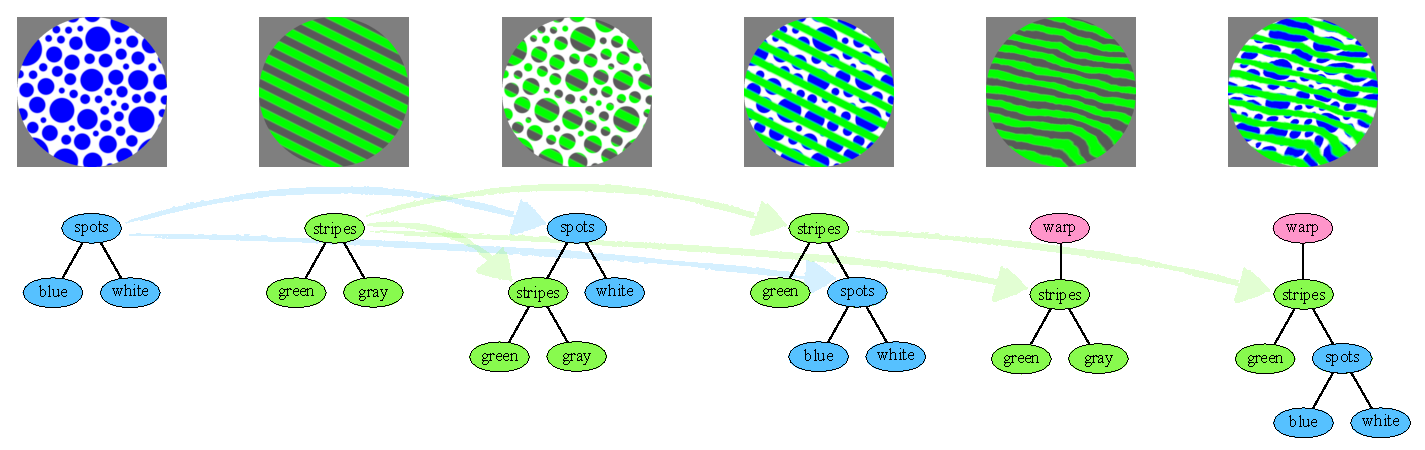
\includegraphics[width=\textwidth]{images/texsyn_overview.pdf}
%     \caption{TexSyn expression trees and crossover between them. A simplified TexSyn with three texture operators (\texttt{spots}, \texttt{stripes}, and \texttt{warp}) plus four unifrom color textures. The first two are minimal trees. The second two show \textit{crossover} between the first two trees, where one leaf is replaced with another tree. The last two show trees with the \texttt{warp} operator applied to example 2 and 4.}
%     \Description{Overview of TexSyn representation of texture and the idea of \textit{crossover} between expression trees.}
%     \label{fig:TexSyn_overview}
% \end{figure*}

\begin{figure*}
    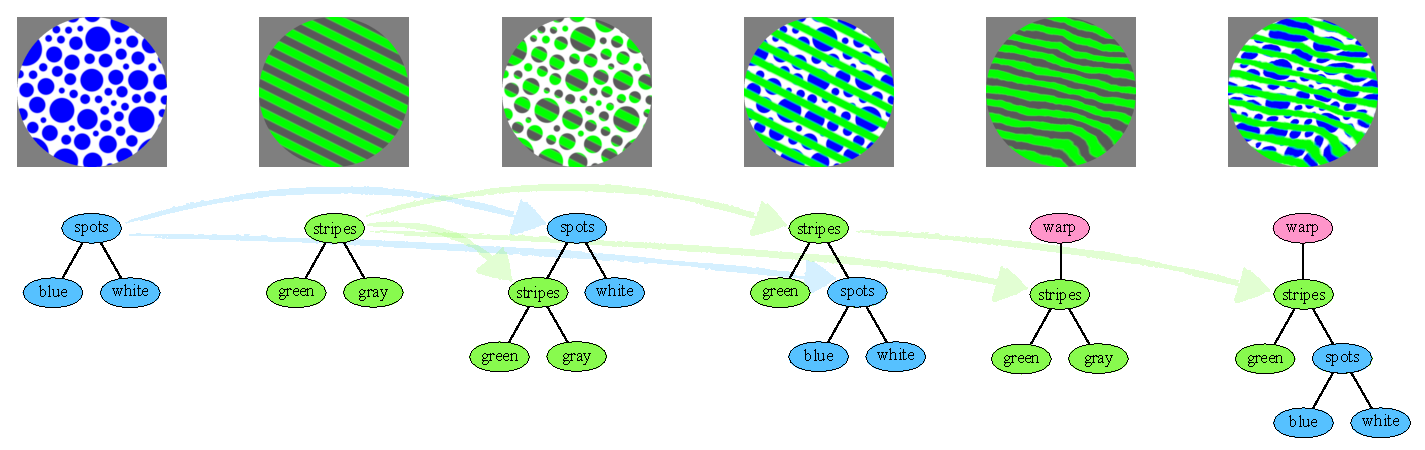
\includegraphics[width=\textwidth]{images/texsyn_overview.pdf}
    \caption{TexSyn expression trees and crossover between them, illustrated with a simplified version of TexSyn with three texture operators (\texttt{spots}, \texttt{stripes}, and \texttt{warp}) plus four color textures. Minimal operator trees are shown in \textit{a} and \textit{b}. \textit{Crossover} between \textit{a} and \textit{b} is shown in \textit{c} and \textit{d}. \textit{c} is \texttt{spots} where \texttt{blue} is replaced with \texttt{stripes}. \textit{d} is \texttt{stripes} where \texttt{gray} is replaced with \texttt{spots}. \textit{e} and \textit{f} show \textit{c} and \textit{d} spliced under \texttt{warp}. (See actual TexSyn c++ code for these examples in Supplemental Materials.)}
    \Description{Overview of TexSyn representation of texture and the idea of \textit{crossover} between expression trees.}
    \label{fig:TexSyn_overview}
\end{figure*}

%% maybe mode detail about GP and TexSyn in appendix? I think that does not add to page count

\section{Discussion}

\section{Limitations}
[... no objective measure of camouflage effectiveness ...]
\par
[... all results are hand selected, “cherry picked” ...] 
\par
[... cite that fast growing literature on “camouflaged object detection” ...]
\par
[... propose a crowd sourced user study of camouflage quality ... could be based on time to find ... like the interactive web games of \href{https://www.visual-ecology.com/2020/10/06/martin-stevens/}{Martin Stevens} nuthatch egg? ...] 
\par
[... in email to Ken I wrote: \textit{The aspect of my project I'm unsure how to approach is lack of rigor. My evaluations are all subjective. It comes down to “we can see that the effectiveness of the camouflage clearly increases during the simulation.”}]
\par
[... inherently 2d ...]
\par
[... texture synthesis lacks genetic or biological plausibility ...]

\section{Future Work}

%% Acknowledgements
\begin{acks}
[... Many thanks to all who helped me with this work: my supportive family, Andrew Glassner for teaching me everything I know about deep learning \cite{glassner_deep_2021}, Ken Perlin for, lots, but especially \cite{perlin_image_1985}. Pat Hanrahan for helpful career advice (“just do the research”). ...]
\par
[... I've been working on this on and off since 2007, based on inspirations by papers in the early 1990s (Witkin/Kass, Turk, Angeline/Pollack, Sims) ...]
\par
[maybe just names (roughly backward in time): 
Ken Perlin,
Aaron Hertzmann,
Andrew Glassner,
Pat Hanrahan,
Karl Sims,
John Koza,
Richard Dawkins,
Witkin/Kass/Turk,
Peter Angeline,
Jordan Pollack.
and of course, Alan Turing. [too weird/maudlin? QQQ]
]
\end{acks}


%% Bibliography.
\bibliographystyle{ACM-Reference-Format}
\bibliography{coc.bib}


%% Appendix
\newpage
\appendix
\section{Supplemental Materials}

Code for Figure \ref{fig:TexSyn_overview} in c++ using TexSyn library:
% \texttt{Uniform white(1);}\par
% \texttt{Uniform gray10(0.1);}\par
% \texttt{Uniform blue(0, 0, 1);}\par
% \texttt{Uniform green(0, 1, 0);}\par
% \texttt{Grating stripes(Vec2(), green, Vec2(0.1, 0.2), gray10, 0.3, 0.5);}\par
% \texttt{LotsOfSpots spots(0.9, 0.05, 0.3, 0.02, 0.02, blue, white);}\par
% \texttt{NoiseWarp warp_stripes(1, 0.1, 0.7, stripes);}\par
% \texttt{LotsOfSpots spots2(0.9, 0.05, 0.3, 0.02, 0.02, stripes, white);}\par
% \texttt{Grating stripes2(Vec2(), green, Vec2(0.1, 0.2), spots, 0.3, 0.5);}\par
% \texttt{NoiseWarp warp_all(1, 0.1, 0.7, stripes2);}\par

% QQQ

% \texttt{Uniform white(1);\par}
% \texttt{Uniform gray(0.1);\par}
% \texttt{Uniform blue(0, 0, 1);\par}
% \texttt{Uniform green(0, 1, 0);\par}
% \texttt{LotsOfSpots spots(0.9, 0.05, 0.3, 0.02, 0.02,\par}
% \texttt{                  blue, white);\par}
% \texttt{Grating stripes(Vec2(), green,\par}
% \texttt{                Vec2(0.1, 0.2), gray,\par}
% \texttt{                0.3, 0.5);\par}
% \texttt{NoiseWarp warp\_stripes(1, 0.1, 0.7, stripes);\par}
% \texttt{LotsOfSpots spots2(0.9, 0.05, 0.3, 0.02, 0.02,\par}
% \texttt{                   stripes, white);\par}
% \texttt{Grating stripes2(Vec2(), green,\par}
% \texttt{                 Vec2(0.1, 0.2), spots,\par}
% \texttt{                 0.3, 0.5);\par}
% \texttt{NoiseWarp warp\_all(1, 0.1, 0.7, stripes2);\par}

\begin{verbatim}
Uniform white(1);
Uniform gray(0.1);
Uniform blue(0, 0, 1);
Uniform green(0, 1, 0);
LotsOfSpots spots(0.9, 0.05, 0.3, 0.02, 0.02,
                  blue, white);
Grating stripes(Vec2(), green,
                Vec2(0.1, 0.2), gray,
                0.3, 0.5);
NoiseWarp warp_stripes(1, 0.1, 0.7, stripes);
LotsOfSpots spots2(0.9, 0.05, 0.3, 0.02, 0.02,
                   stripes, white);
Grating stripes2(Vec2(), green,
                 Vec2(0.1, 0.2), spots,
                 0.3, 0.5);
NoiseWarp warp_all(1, 0.1, 0.7, stripes2);
\end{verbatim}


% Note (from https://s2022.siggraph.org/technical-papers-submissions-faq/): 
% The Conference Paper track encourages submissions for high-quality, 
% ground-breaking research that fits within a strict 7-page limit (plus 
% additional pages for references), and may be more appropriate for
% research that is less-polished but still potentially-impactful. Journal 
% papers do not have a page limit, and may include more thorough experiments
% and derivations within the main paper. 

\end{document}
